\documentclass[xcolor=dvipsnames]{beamer}
\usepackage{lmodern}
\usepackage[T1]{fontenc}
\usepackage[english]{babel}
\usepackage[utf8]{inputenc}

\usepackage{manfnt}
\usepackage{wasysym}
\usepackage{listings}
\usepackage{graphicx}
\usepackage{url}
\usepackage{ulem}
\usepackage{marvosym}
\usepackage{skull}
\usepackage{proof}
\usepackage{array}
\setbeamertemplate{navigation symbols}{}

\title[Dynamic Scheduling in Halide]{{\bf Dynamic Scheduling in Halide}}
\subtitle[]{ {\em cache rules everything around me}}
\author[Ben Blum]{Ben Blum \texttt{(bblum@andrew.cmu.edu)}}

\institute[CMU]{Carnegie Mellon University}
\date[]{2013, December 16}

\setbeamertemplate{footline}{\hspace*{.5cm}\scriptsize{\insertauthor\hspace*{50pt} \hfill\insertframenumber\hspace*{.5cm}}} 

\usecolortheme{seahorse}
\usecolortheme{rose}
\useoutertheme{infolines}

\usecolortheme[named=RoyalBlue]{structure}

\newcommand\noob{\mathsf{noob}}
\newcommand\gibs{\mathsf{gibs}}
\newcommand\dps{\mathsf{dps}}
\newcommand\squig\rightsquigarrow
\newcommand\Coloneqq{\mathrel{\mathop{::}}=}
\newcommand\dmg{\text{\Laserbeam}}
\newcommand\delter\delta
\newcommand\alpher\alpha
\newcommand\defnor{\text{ }|\text{ }}

\newcommand\pimp{\mathop{\supset}}
\newcommand\pand{\mathop{\wedge}}
\newcommand\por{\mathop{\vee}}
\newcommand\ptrue{\top}
\newcommand\pfalse{\bot}


\begin{document}
\renewcommand{\inserttotalframenumber}{28}
\normalem
\begin{frame}
	\titlepage
\end{frame}

%%%%%%%%%%%%%%%%%%%%%%%%%%%%%%%%%%%%%%%%%%%%%%%%%%%%%%%%%%%%%%%%%%%%%%%%%%%%%%%%
%%%%%%%%%%%%%%%%%%%%%%%%%%%%%%%%%%%%%%%%%%%%%%%%%%%%%%%%%%%%%%%%%%%%%%%%%%%%%%%%
%%%%%%%%%%%%%%%%%%%%%%%%%%%%%%%%%%%%%%%%%%%%%%%%%%%%%%%%%%%%%%%%%%%%%%%%%%%%%%%%

\newcommand\linegap{\vspace{0.2in}}
\newcommand\breakslide[1]{\begin{frame}{} \begin{center} \Large #1 \end{center} \end{frame}}
\newcommand\related[1]{\textsuperscript{\em [#1]}}
\newcommand\hilight[2]{\color{#1}#2\color{black}}

\begin{frame}{Outline}
	\textbf{Halide Review}
	\begin{itemize}
		\item Function Definitions
		\item Function Scheduling
	\end{itemize}
	\linegap

	{\bf Dynamic Scheduling}
	\begin{itemize}
		\item Problem: Dynamic Vector Fields
		\item Solution: Cache Computed Values
	\end{itemize}
	\linegap

	{\bf Evaluation}
\end{frame}

%%%%%%%%%%%%%%%%%%%%%%%%%%%%%%%%%%%%%%%%%%%%%%%%%%%%%%%%%%%%%%%%%%%%%%%%%%%%%%%%
\section{Halide Review}
%%%%%%%%%%%%%%%%%%%%%%%%%%%%%%%%%%%%%%%%%%%%%%%%%%%%%%%%%%%%%%%%%%%%%%%%%%%%%%%%

\newcommand\code[1]{{\begin{center}\fbox{\begin{tabular}{l} #1 \end{tabular}} \end{center}}}

\definecolor{grey}{RGB}{127,127,127}
\definecolor{darkcyan}{RGB}{0,127,127}
\definecolor{olivegreen}{RGB}{0,127,0}
\definecolor{violet}{RGB}{127,0,127}
\definecolor{brickred}{RGB}{127,0,0}
\definecolor{brown}{RGB}{127,63,0}
\definecolor{orange}{RGB}{192,96,0}

\begin{frame}{Image Processing is Functional Programming}
	\begin{columns}

	\column{0.5\textwidth}
	\begin{tabular}{l}
		\texttt{blur\_y(x,y) =} \\
		\texttt{~~~~(input(x, y-1) +}\\
		\texttt{~~~~~input(x, y~~) +}\\
		\texttt{~~~~~input(x, y+1))/3;}\\
		\\
		\\
		\\
		\\
		\\
	\end{tabular}

	\column{0.5\textwidth}
	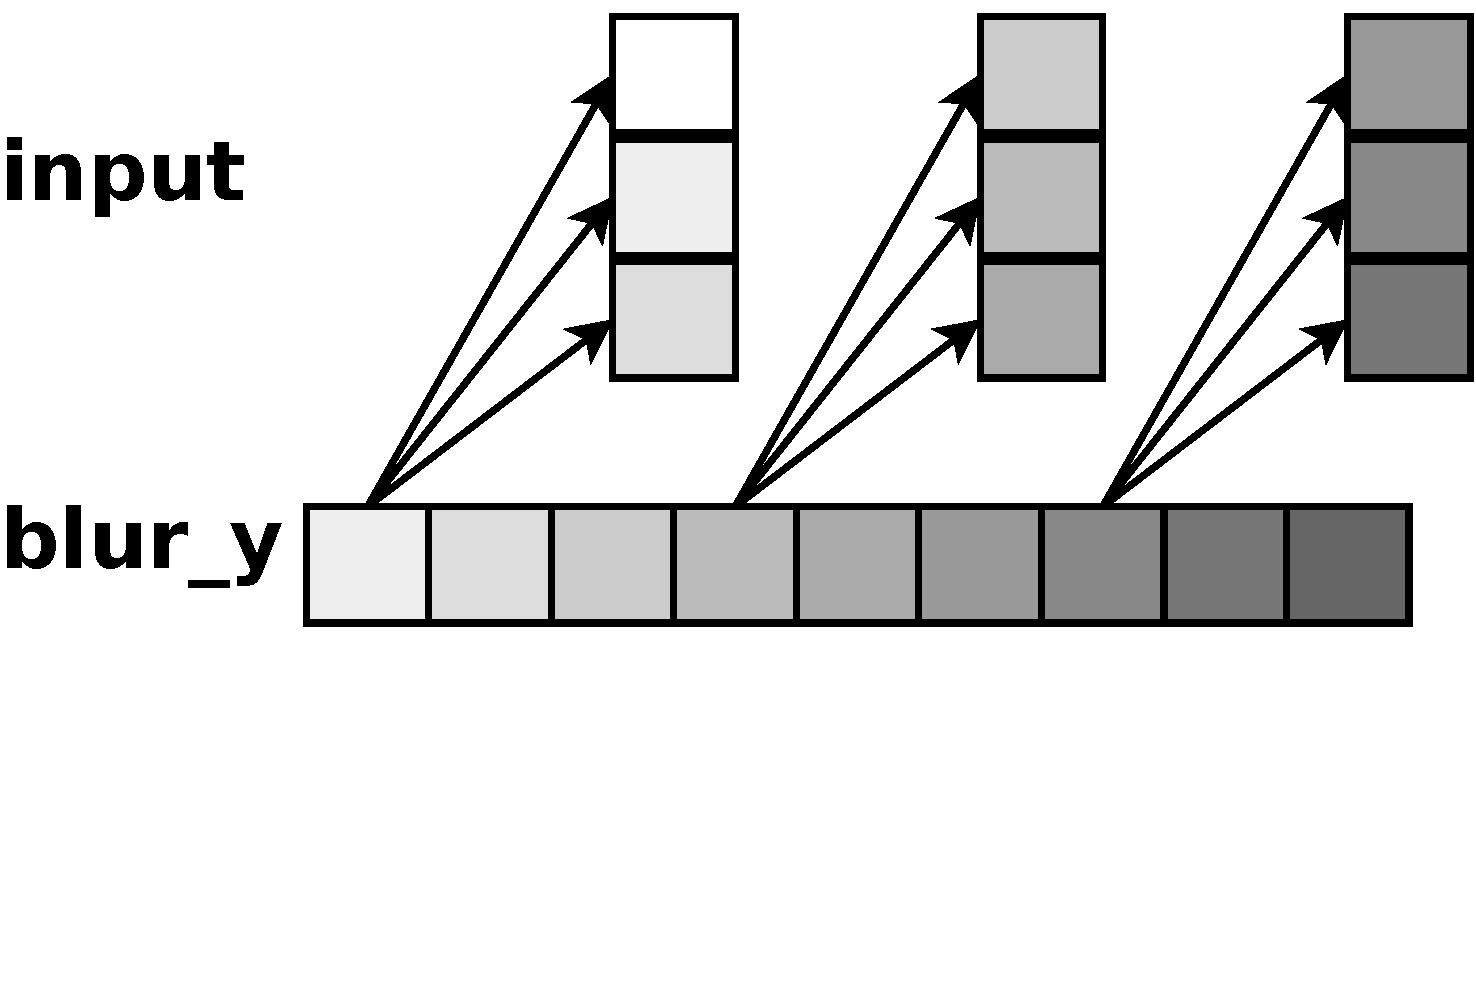
\includegraphics[width=\textwidth]{blury.pdf}
	\end{columns}
\end{frame}

\begin{frame}{Image Processing is Functional Programming}
	\begin{columns}

	\column{0.5\textwidth}
	\begin{tabular}{l}
		\texttt{blur\_y(x,y) =} \\
		\texttt{~~~~(input(x, y-1) +}\\
		\texttt{~~~~~input(x, y~~) +}\\
		\texttt{~~~~~input(x, y+1))/3;}\\
		\\
		\texttt{blur\_x(x,y) =} \\
		\texttt{~~~~(blur\_y(x-1, y) +}\\
		\texttt{~~~~~blur\_y(x,~~~y) +}\\
		\texttt{~~~~~blur\_y(x+1, y))/3;}\\
	\end{tabular}

	\column{0.5\textwidth}
	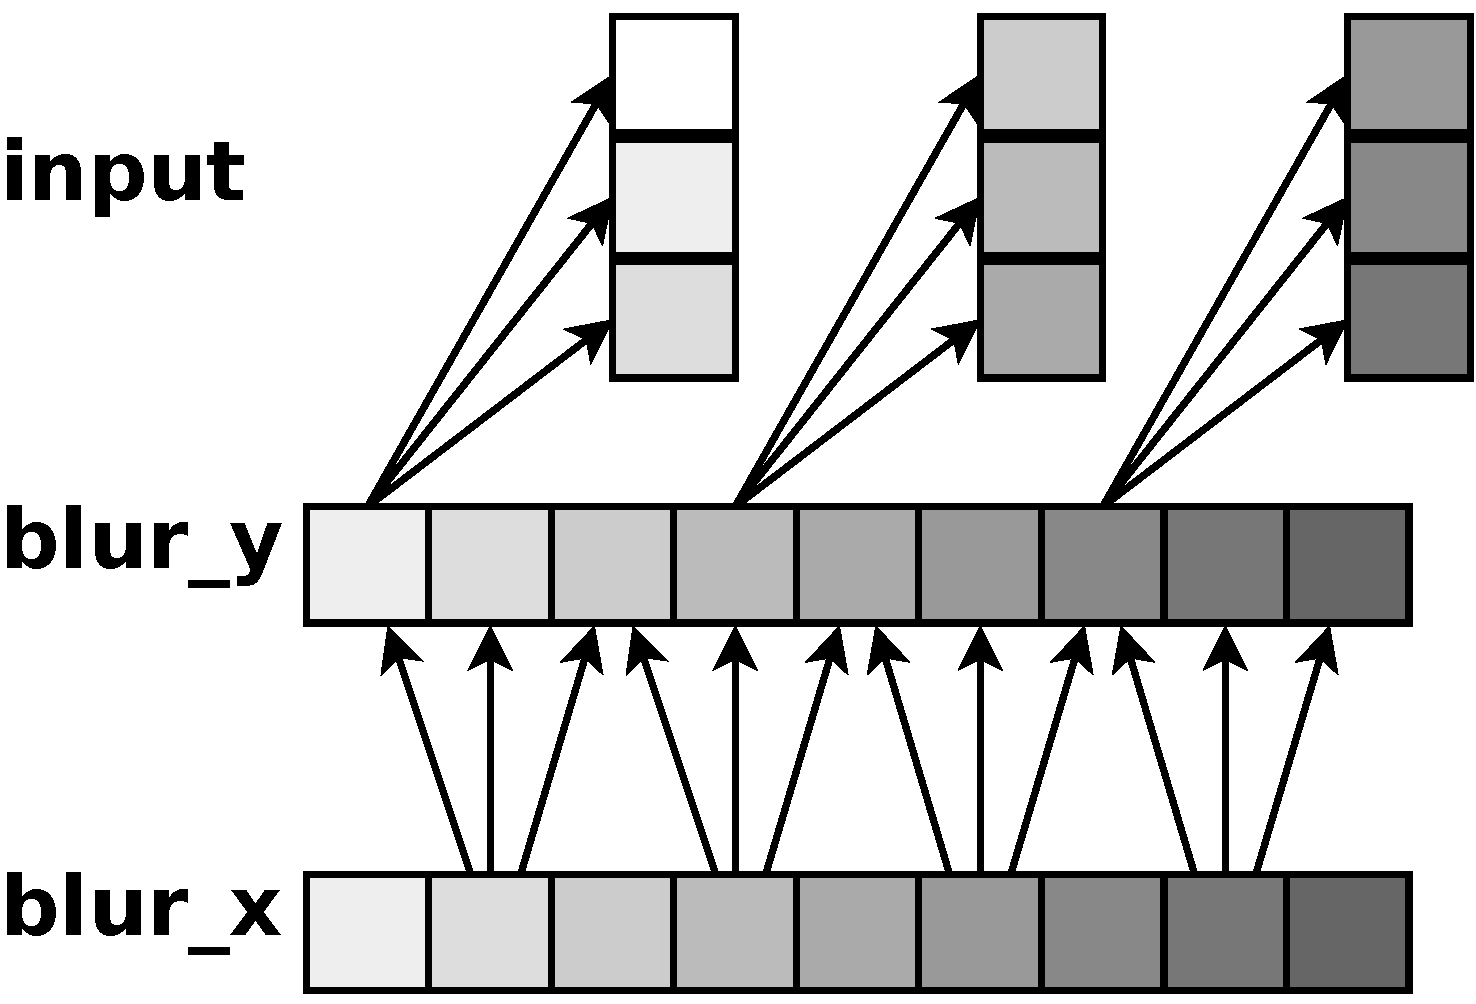
\includegraphics[width=\textwidth]{blurx.pdf}
	\end{columns}
\end{frame}

\begin{frame}{...embedded in C++}
	\begin{tabular}{l}
		\\
		\\
		\\
		\\
		\\
		\texttt{void main(int argc, char **argv)}\\
		\texttt{~~~~Image<float> \hilight{blue}{input}~= load(argv[1]);} \\
		\texttt{~~~~Image<float> output(input.width(), input.height());}\\
		\texttt{~~~~Func \hilight{blue}{blur\_y}, \hilight{blue}{blur\_x};} \\
		\texttt{~~~~Var \hilight{blue}{x},\hilight{blue}{y};}\\
		\texttt{~~~~\hilight{blue}{blur\_y(x,y) = (input(x, y-1) + ...)/3;}} \\
		\texttt{~~~~\hilight{blue}{blur\_x(x,y) = (blur\_y(x-1, y) + ...)/3;}} \\
		\\
		\texttt{~~~~\hilight{blue}{blur\_x}.realize(output); // JITs and runs the blur} \\
		\texttt{~~~~save(output, "output.png");} \\
		\texttt{\}}\\
	\end{tabular}
\end{frame}

\begin{frame}{...embedded in C++}
	\begin{tabular}{l}
		\texttt{class Expr \{ ... \};}\\
		\texttt{class Func \{}\\
		\texttt{~~~~operator()(Expr x, Expr y, Expr z, ...);}\\
		\texttt{~~~~...}\\
		\texttt{\};}\\
		\texttt{void main(int argc, char **argv)}\\
		\texttt{~~~~Image<float> \hilight{blue}{input}~= load(argv[1]);} \\
		\texttt{~~~~Image<float> output(input.width(), input.height());}\\
		\texttt{~~~~Func \hilight{blue}{blur\_y}, \hilight{blue}{blur\_x};} \\
		\texttt{~~~~Var \hilight{blue}{x},\hilight{blue}{y};}\\
		\texttt{~~~~\hilight{blue}{blur\_y(x,y) = (input(x, y-1) + ...)/3;}} \\
		\texttt{~~~~\hilight{blue}{blur\_x(x,y) = (blur\_y(x-1, y) + ...)/3;}} \\
		\\
		\texttt{~~~~\hilight{blue}{blur\_x}.realize(output); // JITs and runs the blur} \\
		\texttt{~~~~save(output, "output.png");} \\
		\texttt{\}}\\
	\end{tabular}
\end{frame}

\begin{frame}{Functions are Automatically ``Scheduled''}
	\begin{columns}

	\column{0.4\textwidth}
	\begin{tabular}{l}
		\texttt{\hilight{olivegreen}{blur\_y(x,y) =}} \\
		\texttt{\hilight{olivegreen}{~~(input(x, y-1) +}}\\
		\texttt{\hilight{olivegreen}{~~~input(x, y,~~~c) +}}\\
		\texttt{\hilight{olivegreen}{~~~input(x, y+1))/3;}}\\
		\\
		\texttt{\hilight{blue}{blur\_x(x,y) =}} \\
		\texttt{\hilight{blue}{~~(blur\_y(x-1, y) +}}\\
		\texttt{\hilight{blue}{~~~blur\_y(x,~~~y) +}}\\
		\texttt{\hilight{blue}{~~~blur\_y(x+1, y))/3;}}\\
		\\
		\\
		\\
	\end{tabular}

	\column{0.05\textwidth}
	\column{0.55\textwidth}
		\texttt{\hilight{olivegreen}{float~blur\_y[HEIGHT][WIDTH];}} \\
		\texttt{\hilight{olivegreen}{for~(row~=~0~to~HEIGHT)~\{}} \\
		\texttt{\hilight{olivegreen}{~~for~(col~=~0~to~WIDTH)~\{}} \\
		\texttt{\hilight{olivegreen}{~~~~blur\_y[row][col] = ...;}}\\
		\texttt{\hilight{olivegreen}{~~\}}} \\
		\texttt{\hilight{olivegreen}{\}}} \\
		\texttt{\hilight{blue}{float~blur\_x[HEIGHT][WIDTH];}} \\
		\texttt{\hilight{blue}{for~(row~=~0~to~HEIGHT)~\{}} \\
		\texttt{\hilight{blue}{~~for~(col~=~0~to~WIDTH)~\{}} \\
		\texttt{\hilight{blue}{~~~~blur\_x[row][col] = ...;}}\\
		\texttt{\hilight{blue}{~~\}}} \\
		\texttt{\hilight{blue}{\}}} \\
	\end{columns}
	\pause
	\begin{itemize}
		\item Bad locality: Traversing the whole image twice
		\item Bad paralellism: One thread per row/column/pixel??
	\end{itemize}
\end{frame}

\begin{frame}{Function Schedules Can Be Configured}
	\begin{tabular}{l}
		{\bf \texttt{blur\_x.tile(x, y, x2, y2, 8, 8).parallel(x, y);}}\\
		{\bf \texttt{blur\_y.store\_at(blur\_x, x).compute\_at(blur\_x, y2);}}\\
		\\
		\\
		\\
		\\
		\\
		\\
		\\
		\\
		\\
		\\
		\\
		\\
		\\
		\\
		\\
	\end{tabular}
\end{frame}

\begin{frame}{Function Schedules Can Be Configured}
	\begin{tabular}{l}
		{\bf \texttt{blur\_x.tile(x, y, x2, y2, 8, 8).parallel(x, y);}}\\
		{\bf \texttt{blur\_y.store\_at(blur\_x, x).compute\_at(blur\_x, y2);}}\\
		\\
		\texttt{\hilight{blue}{float~blur\_x[HEIGHT][WIDTH];}} \\
		\texttt{\hilight{blue}{PARALLEL for~(row~=~0~to~8)~\{}} \\
		\texttt{\hilight{blue}{~~PARALLEL for~(col~=~0~to~8)~\{}} \\
		\texttt{\hilight{olivegreen}{~~~~float~blur\_y[HEIGHT/8][WIDTH/8];}} \\
		\texttt{\hilight{blue}{~~~~for~(row2~=~0~to~WIDTH/8)~\{}} \\
		\texttt{\hilight{olivegreen}{~~~~~~for~(col2~=~0~to~WIDTH/8)~\{}} \\
		\texttt{\hilight{olivegreen}{~~~~~~~~blur\_y[row*8~+~row2][col*8~+~col2]~=~...;}} \\
		\texttt{\hilight{olivegreen}{~~~~~~\}}} \\
		\texttt{\hilight{blue}{~~~~~~for~(col2~=~0~to~WIDTH/8)~\{}} \\
		\texttt{\hilight{blue}{~~~~~~~~blur\_x[row*8~+~row2][col*8~+~col2]~=~...;}} \\
		\texttt{\hilight{blue}{~~~~~~\}}} \\
		\texttt{\hilight{blue}{~~~~\}}} \\
		\texttt{\hilight{blue}{~~\}}} \\
		\texttt{\hilight{blue}{\}}} \\
	\end{tabular}
\end{frame}

\begin{frame}{Function Schedules Can Be Configured}
	\begin{tabular}{l}
		{\bf \texttt{blur\_x.tile(x, y, x2, y2, 8, 8).parallel(x, y);}}\\
		{\bf \texttt{blur\_y.store\_at(blur\_x, x).compute\_at(blur\_x, y2);}}\\
		\\
		\texttt{\hilight{blue}{float~blur\_x[HEIGHT][WIDTH];}} \\
		\texttt{\hilight{blue}{PARALLEL for~(row~=~0~to~8)~\{}} \quad {\bf // Good parallelism} \\
		\texttt{\hilight{blue}{~~PARALLEL for~(col~=~0~to~8)~\{}} \\
		\texttt{\hilight{olivegreen}{~~~~float~blur\_y[HEIGHT/8][WIDTH/8];}} \quad {\bf // Low memory usage} \\
		\texttt{\hilight{blue}{~~~~for~(row2~=~0~to~WIDTH/8)~\{}} \\
		\texttt{\hilight{olivegreen}{~~~~~~for~(col2~=~0~to~WIDTH/8)~\{}} \quad {\bf // Good locality} \\
		\texttt{\hilight{olivegreen}{~~~~~~~~blur\_y[row*8~+~row2][col*8~+~col2]~=~...;}} \\
		\texttt{\hilight{olivegreen}{~~~~~~\}}} \\
		\texttt{\hilight{blue}{~~~~~~for~(col2~=~0~to~WIDTH/8)~\{}} \\
		\texttt{\hilight{blue}{~~~~~~~~blur\_x[row*8~+~row2][col*8~+~col2]~=~...;}} \\
		\texttt{\hilight{blue}{~~~~~~\}}} \\
		\texttt{\hilight{blue}{~~~~\}}} \\
		\texttt{\hilight{blue}{~~\}}} \\
		\texttt{\hilight{blue}{\}}} \\
	\end{tabular}
\end{frame}

\begin{frame}{Tiling Helps Parallelism and Locality}
	\begin{center}
	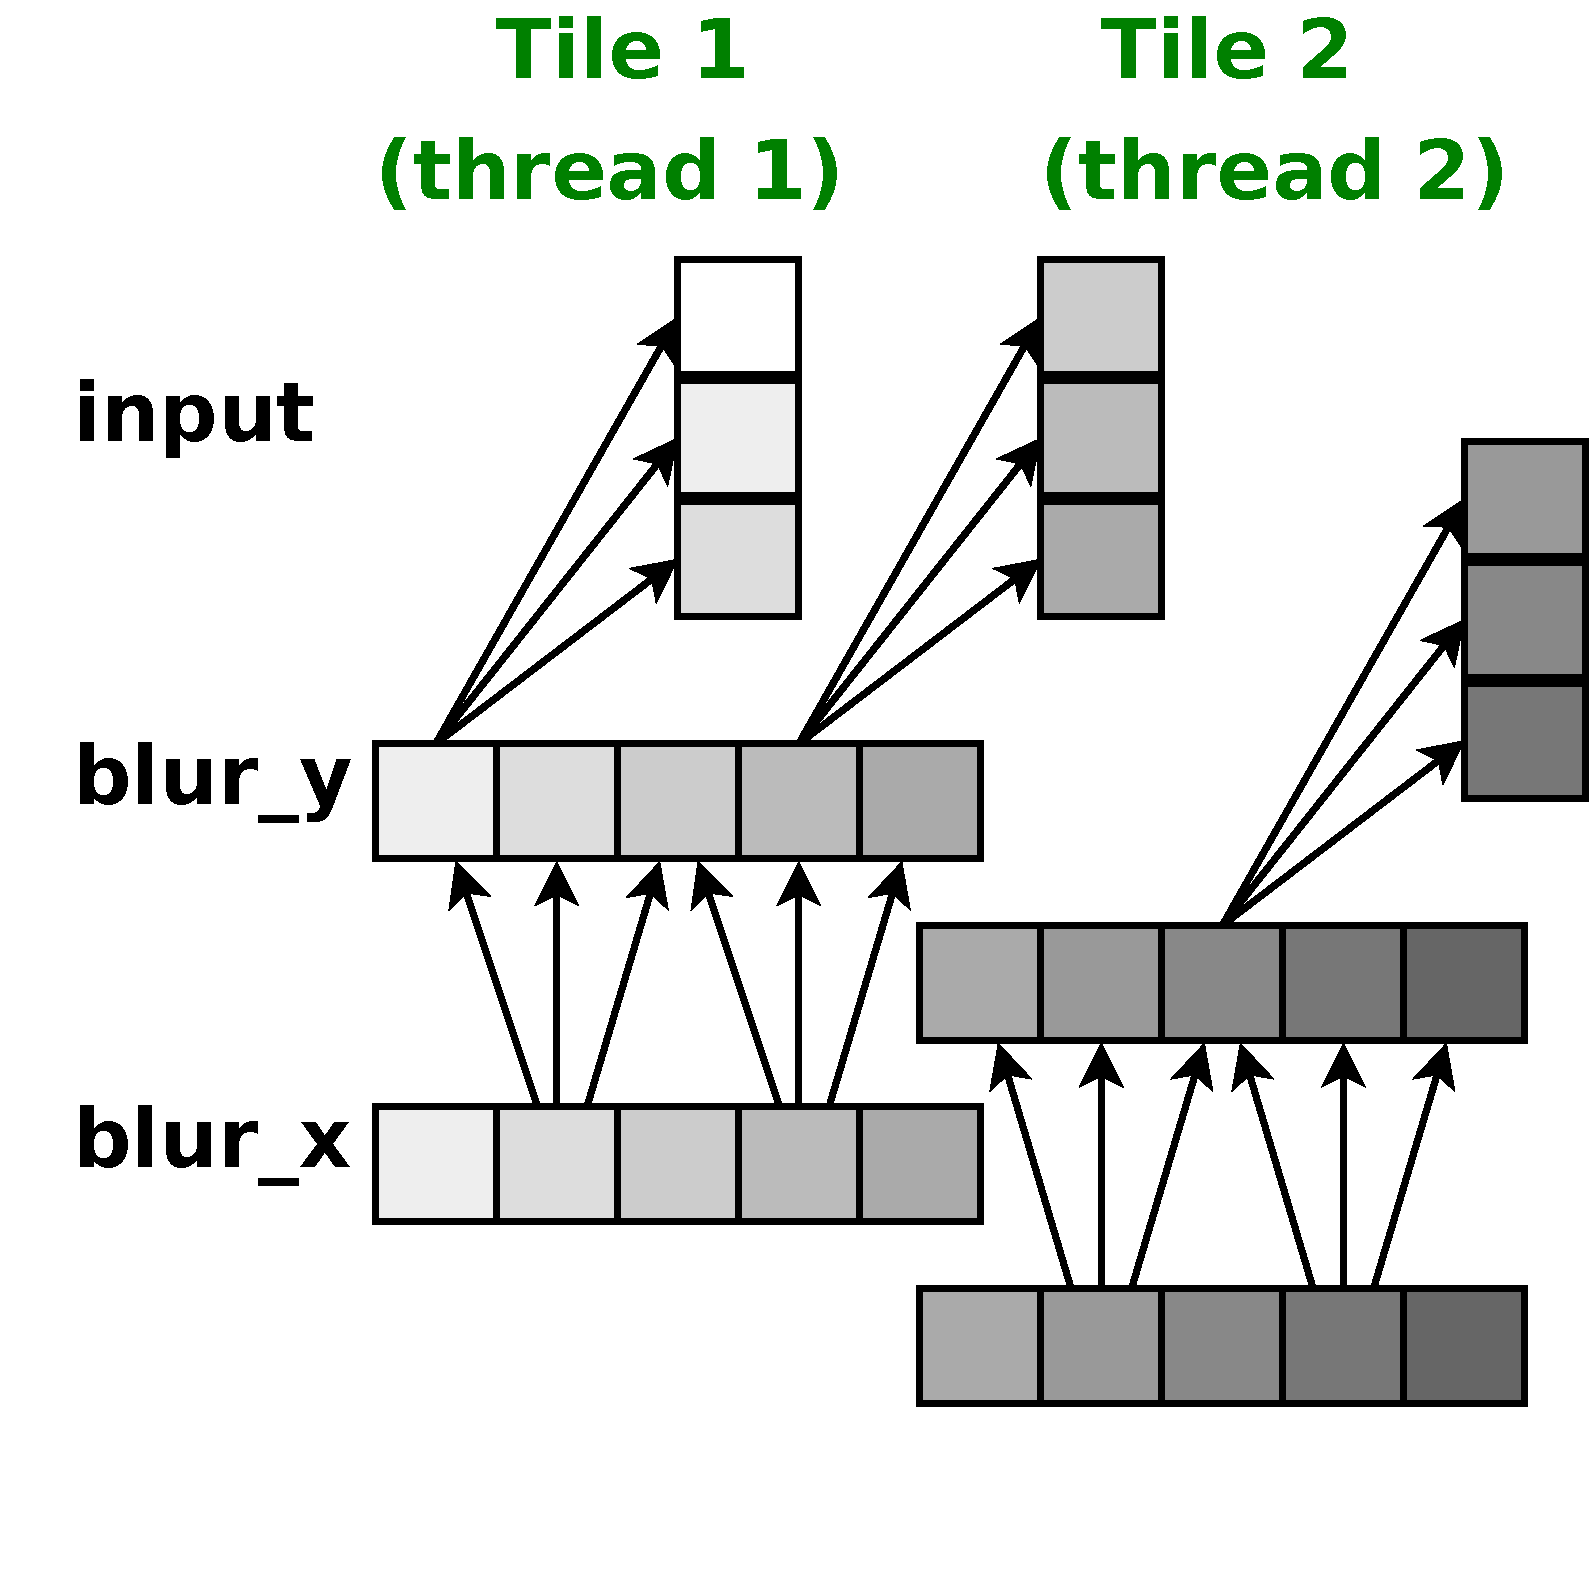
\includegraphics[width=0.6\textwidth]{blur-tile.pdf}
	\end{center}
\end{frame}

\begin{frame}{Tiling Helps Parallelism and Locality}
	\begin{center}
	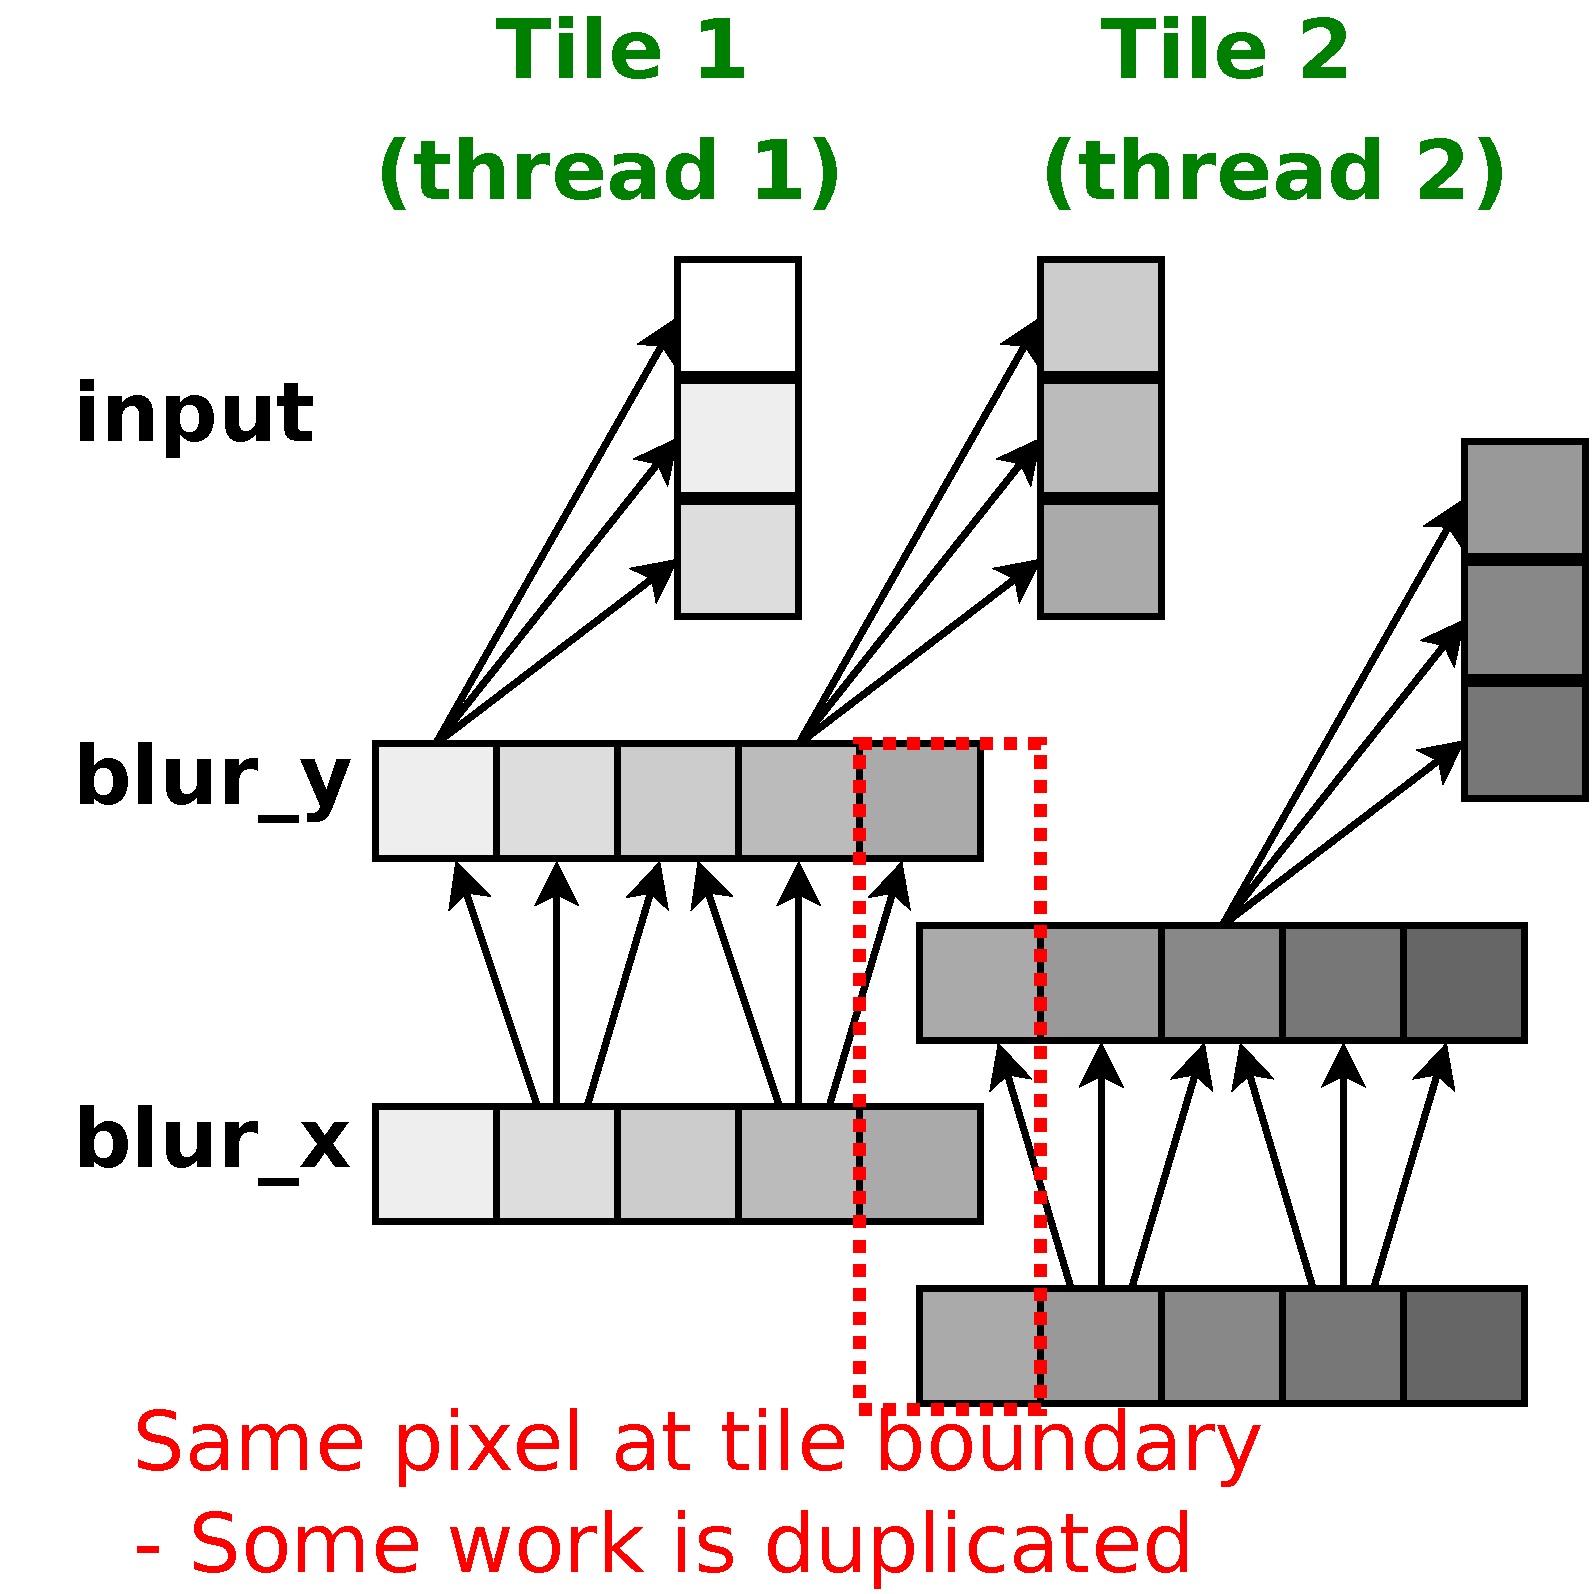
\includegraphics[width=0.6\textwidth]{blur-tile2.pdf}
	\end{center}
\end{frame}


%float blur_x[HEIGHT][WIDTH];
%for (row = 0 to 8) {
%  for (col = 0 to 8) {
%    float blur_y[HEIGHT/8][WIDTH/8];
%    for (row2 = 0 to WIDTH/8) {
%      for (col2 = 0 to WIDTH/8) {
%        blur_y[row*8 + row2][col*8 + col2] = ...;
%      }
%      for (col2 = 0 to WIDTH/8) {
%        blur_x[row*8 + row2][col*8 + col2] = ...;
%      }
%    }
%  }
%}

%float blur_x[HEIGHT][WIDTH];
%for (blur_x_row = 0 to HEIGHT) {
%  float blur_y[WIDTH];
%  for (blur_y_col = 0 to WIDTH) {
%    blur_y[blur_y_col] = ...;
%  }
%  for (blur_x_col = 0 to WIDTH) {
%    blur_x[blur_x_col] = ...;
%  }
%}

%%%%%%%%%%%%%%%%%%%%%%%%%%%%%%%%%%%%%%%%%%%%%%%%%%%%%%%%%%%%%%%%%%%%%%%%%%%%%%%%
\section{Dynamic Scheduling}
%%%%%%%%%%%%%%%%%%%%%%%%%%%%%%%%%%%%%%%%%%%%%%%%%%%%%%%%%%%%%%%%%%%%%%%%%%%%%%%%

\breakslide{Dynamic Scheduling}

\begin{frame}{Static vs Dynamic Data Dependencies}
	Avoiding duplicate work when tiling relies on {\bf static data dependencies}.
	\begin{itemize}
		\item In 3x3 blur, max distance from output to input location was 1.
	\end{itemize}
	\linegap

	However, some algorithms compute which pixels to read from dynamically.
	\begin{itemize}
		\item Patch-match
		\item Edge detection
	\end{itemize}
	\linegap

	Which input pixels each output pixel will need to compute (the {\bf vector field}) is not known until runtime.
\end{frame}

\begin{frame}{Dynamic Vector Field Example}
	\vspace{-0.3in}
	\begin{center}
	\begin{tabular}{cc}
	\begin{tabular}{c}
	Original image \\
	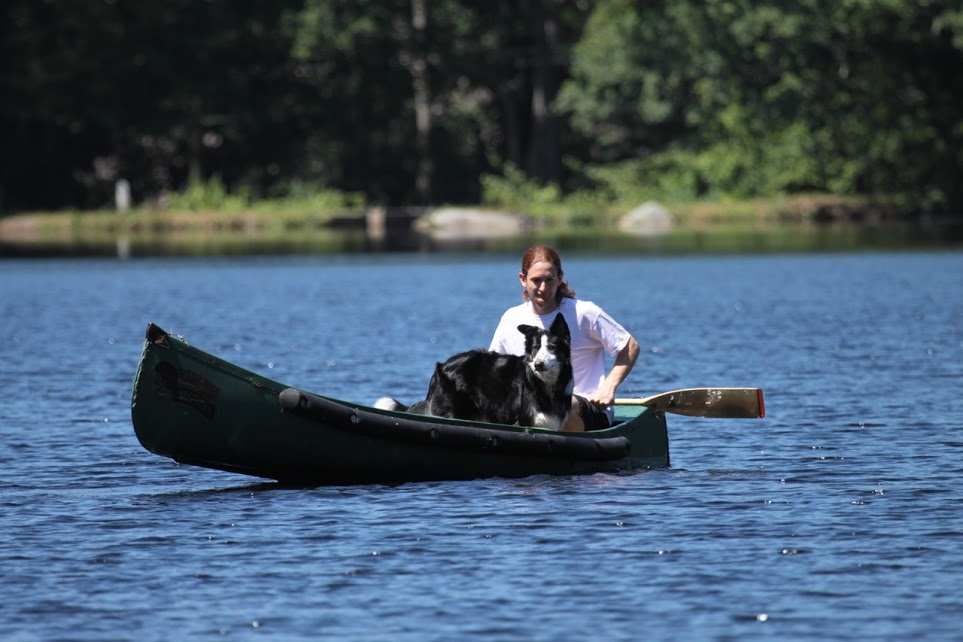
\includegraphics[width=0.40\textwidth]{canoe-0.png}
	\end{tabular}
	& \pause
	\begin{tabular}{c}
	Invert colours  \\
	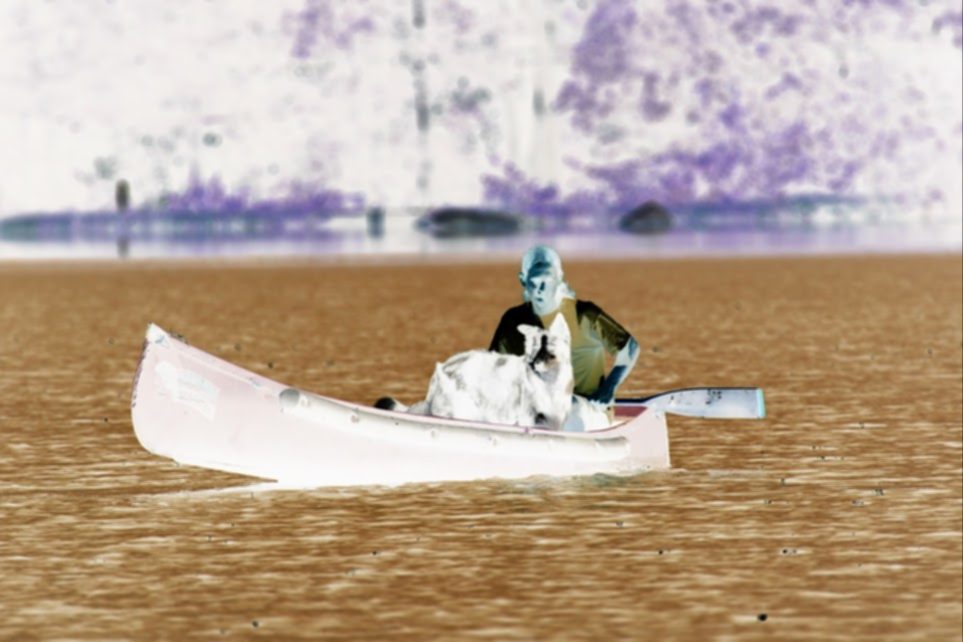
\includegraphics[width=0.40\textwidth]{canoe-1.png}
	\end{tabular}
	\\ \pause
	\begin{tabular}{c}
	Flip \& Blur \\
	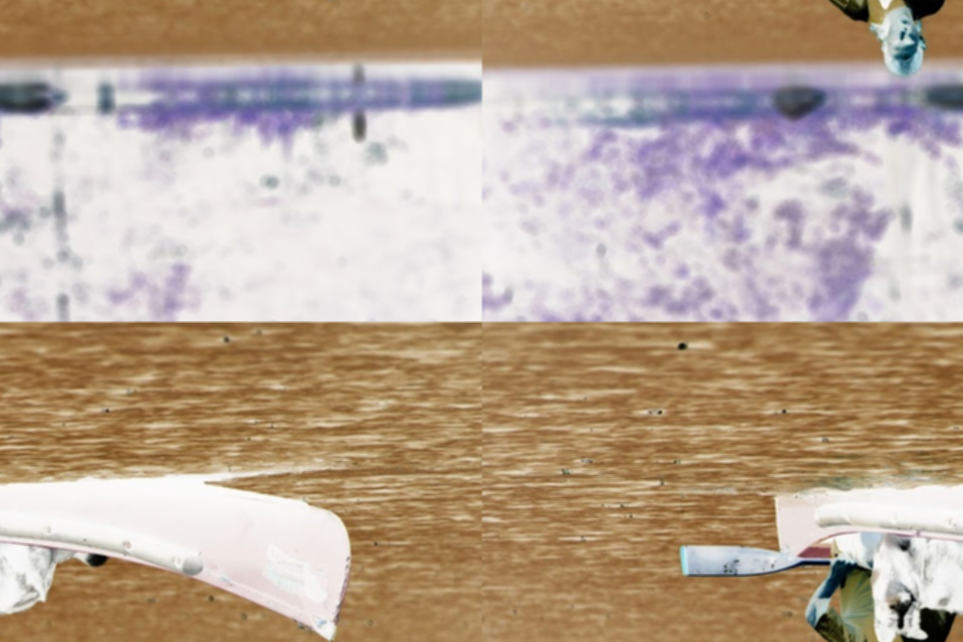
\includegraphics[width=0.40\textwidth]{canoe-2.png}
	\end{tabular}
	& \pause
	\begin{tabular}{c}
	Flip conditionally by colour of pixel \\
	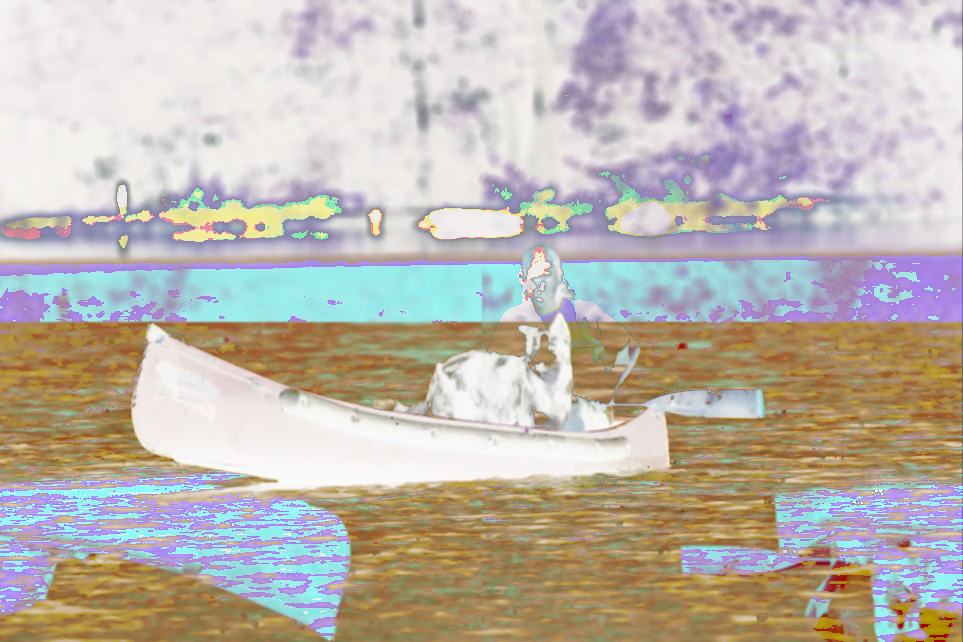
\includegraphics[width=0.40\textwidth]{canoe-3.png}
	\end{tabular}
	\end{tabular}
	\end{center}
\end{frame}
\begin{frame}{Dynamic Vector Fields Cause Duplicate Work}
	\begin{center}
	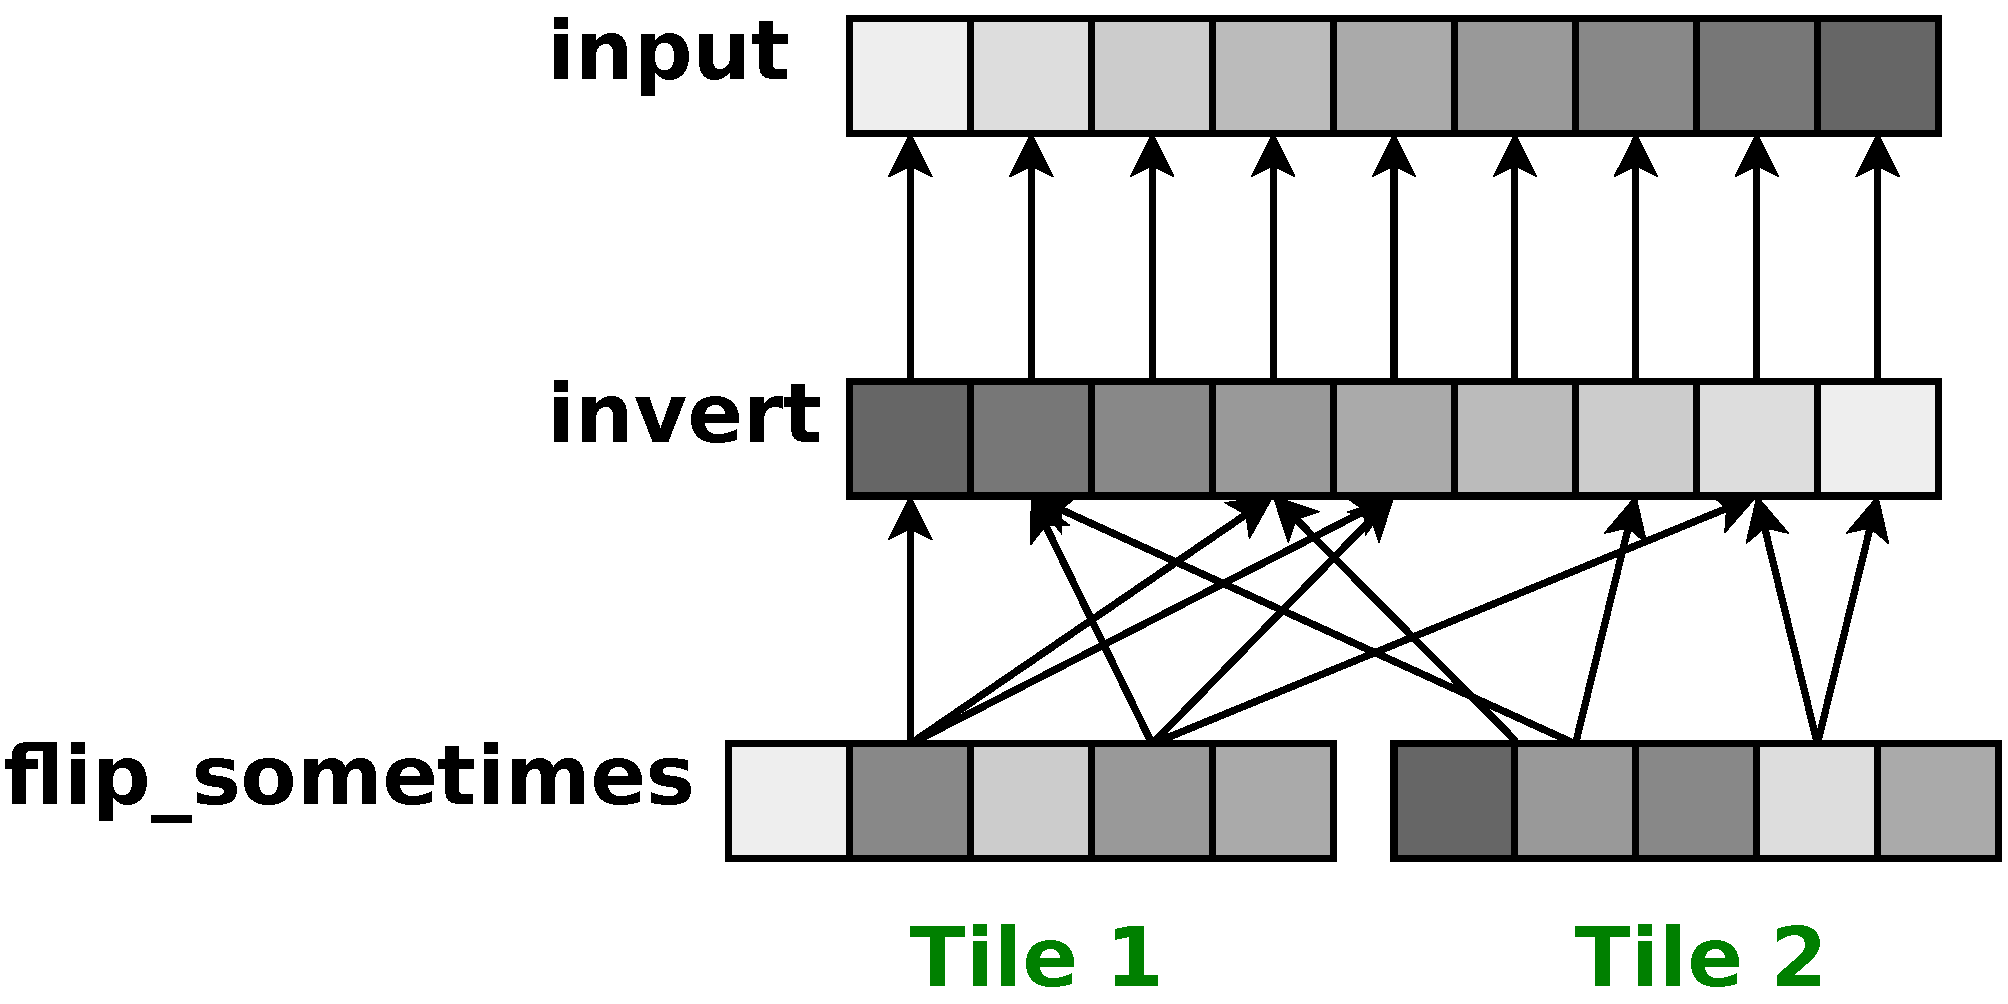
\includegraphics[width=0.7\textwidth]{blur-dynamic.pdf}
	\end{center}
	\pause
	\linegap

	Goal: When tile 1 computes \texttt{invert()} on a pixel, {\bf remember it} for tile 2.
\end{frame}

\begin{frame}{Solution: Caching Computed Results}
	\textbf{Generated code, before:}
	\linegap

	\begin{tabular}{l}
		\\
		\texttt{\hilight{blue}{for~(tile~=~...)~\{}} \quad {\bf // Work duplicated across iterations} \\
		\texttt{\hilight{olivegreen}{~~for~(row~=~...) \{}}\\
		\texttt{\hilight{olivegreen}{~~~~for~(col~=~...) \{}}\\
		\\
		\texttt{\hilight{olivegreen}{~~~~~~~~inverted[row][col]~=~...;}} \\
		\\
		\\
		\texttt{\hilight{olivegreen}{~~~~\}}} \\
		\texttt{\hilight{olivegreen}{~~\}}} \\
		\texttt{\hilight{blue}{~~(... compute flipped ...)}} \\
		\texttt{\hilight{blue}{\}}} \\
	\end{tabular}
\end{frame}

\begin{frame}{Solution: Caching Computed Results}
	\textbf{Generated code, after:}
	\linegap

	\begin{tabular}{l}
		\texttt{\hilight{orange}{bool~result\_computed[...];}}\\
		\texttt{\hilight{blue}{for~(tile~=~...)~\{}} \quad {\bf // Work cached across iterations} \\
		\texttt{\hilight{olivegreen}{~~for~(row~=~...) \{}}\\
		\texttt{\hilight{olivegreen}{~~~~for~(col~=~...) \{}}\\
		\texttt{\hilight{orange}{~~~~~~if (!result\_computed[row][col]) \{}} \\
		\texttt{\hilight{olivegreen}{~~~~~~~~inverted[row][col]~=~...;}} \\
		\texttt{\hilight{orange}{~~~~~~~~result\_computed[row][col]~=~true;}} \\
		\texttt{\hilight{orange}{~~~~~~\}}} \\
		\texttt{\hilight{olivegreen}{~~~~\}}} \\
		\texttt{\hilight{olivegreen}{~~\}}} \\
		\texttt{\hilight{blue}{~~(... compute flipped ...)}} \\
		\texttt{\hilight{blue}{\}}} \\
	\end{tabular}
\end{frame}

%%%%%%%%%%%%%%%%%%%%%%%%%%%%%%%%%%%%%%%%%%%%%%%%%%%%%%%%%%%%%%%%%%%%%%%%%%%%%%%%
\section{Evaluation}
%%%%%%%%%%%%%%%%%%%%%%%%%%%%%%%%%%%%%%%%%%%%%%%%%%%%%%%%%%%%%%%%%%%%%%%%%%%%%%%%

\breakslide{Evaluation}

\begin{frame}{Evaluation}
	Evaluation Questions
	\begin{itemize}
		\item How much duplicate work does this let us avoid?
		\item How do different tilings, etc. affect savings?
	\end{itemize}
	\pause
	\linegap

	Approach
	\begin{itemize}
		\item Used the transformation from the example
		\begin{itemize}
			\item (stage 1 \texttt{invert}, stage 2 \texttt{flip\_and\_blur})
		\end{itemize}
		\item Measured \# of calls to \texttt{invert} and execution time
		\item Tested with several different function schedules
	\end{itemize}
\end{frame}

\begin{frame}{Experimental Setup}
	Ran experiments using small, medium, and large images
	\begin{center}
	\begin{tabular}{ccc}
	\begin{tabular}{c}
	64 x 64 \\
	
\includegraphics{gradient.png} \\
	
\includegraphics{gradient-output.png} \\
	\end{tabular} &
	\begin{tabular}{c}
	400 x 261 \\
	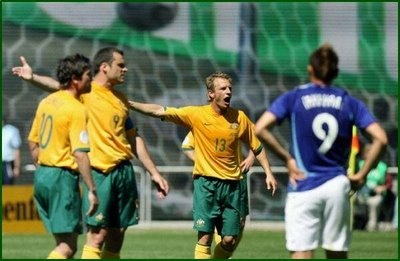
\includegraphics[width=0.3\textwidth]{readers-writers.png} \\
	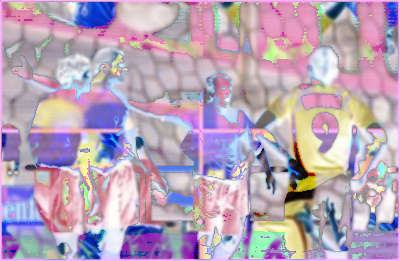
\includegraphics[width=0.3\textwidth]{rw-output.png} \\
	\end{tabular} &
	\begin{tabular}{c}
	963 x 642 \\
	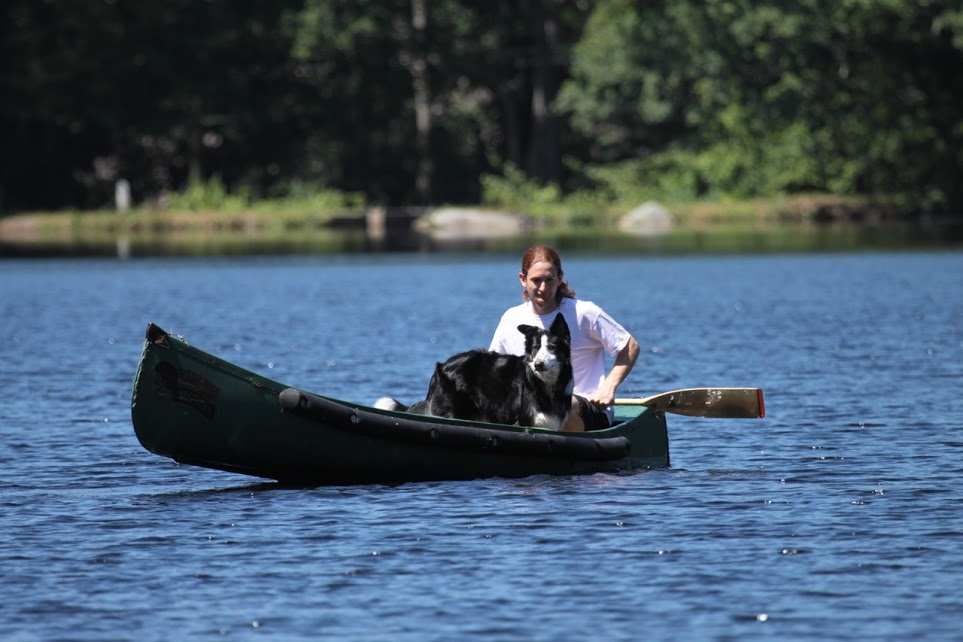
\includegraphics[width=0.3\textwidth]{canoe-0.png} \\
	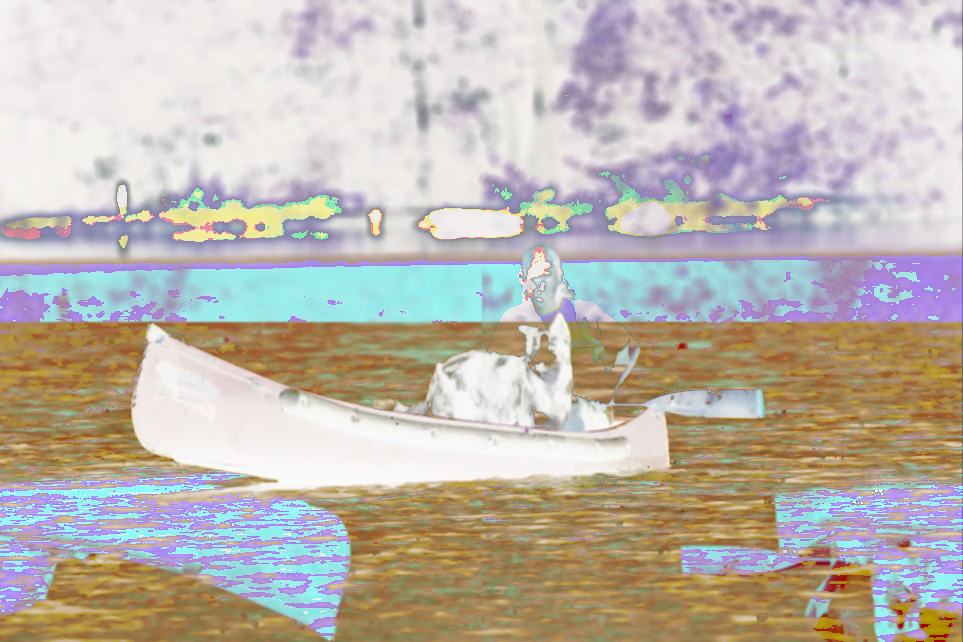
\includegraphics[width=0.3\textwidth]{canoe-3.png} \\
	\end{tabular}
	\end{tabular}
	\end{center}

\end{frame}

\begin{frame}{Result: Dynamic Scheduling Saves Computation}
	For small image, measured number of \texttt{invert()} calls during execution
	\begin{itemize}
		\item (think: number of ``cache misses'')
	\end{itemize}
	\linegap

	\begin{center}
	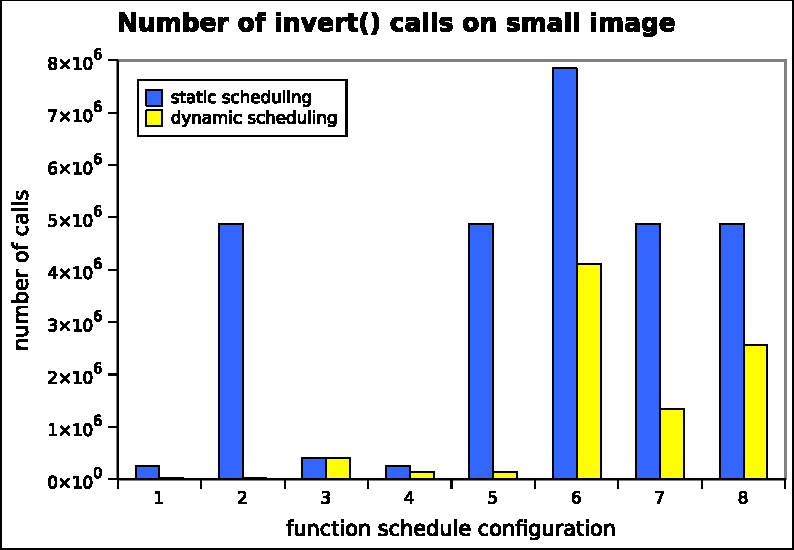
\includegraphics[width=0.7\textwidth]{graphs/small.pdf}
	\end{center}
\end{frame}

%%%%%%%%%%%%%%%%%%%%%%%%%%%%%%%%%%%%%%%%%%%%%%%%%%%%%%%%%%%%%%%%%%%%%%%%%%%%%%%%
\section{Conclusion}
%%%%%%%%%%%%%%%%%%%%%%%%%%%%%%%%%%%%%%%%%%%%%%%%%%%%%%%%%%%%%%%%%%%%%%%%%%%%%%%%

\breakslide{Conclusion}

\begin{frame}{Summary}
	Halide separates {\bf algorithm logic} from {\bf function scheduling}.
	\linegap

	Schedules are influenced by {\bf data dependencies} between algorithm stages.
	\linegap

	\textbf{Dynamically caching results} can succeed where static reasoning fails.
\end{frame}

\begin{frame}{Questions?}
	\begin{center}
	\begin{tabular}{ccc}
	\begin{tabular}{c}
	
\includegraphics[width=0.2\textwidth]{bloopers/01.png} \\
	\\
	
\includegraphics[width=0.2\textwidth]{bloopers/04.png} \\
	\end{tabular} &
	\begin{tabular}{c}
	
\includegraphics[width=0.2\textwidth]{bloopers/02.png} \\
	\\
	
\includegraphics[width=0.2\textwidth]{bloopers/05.png} \\
	\end{tabular} &
	\begin{tabular}{c}
	
\includegraphics[width=0.2\textwidth]{bloopers/03.png} \\
	\\
	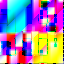
\includegraphics[width=0.2\textwidth]{bloopers/06.png} \\
	\end{tabular}
	\end{tabular}
	\\ \linegap
	(``bloopers'' produced during debugging)
	\end{center}

\end{frame}

\breakslide{Bonus Slides}

\begin{frame}{Open Questions}
	Can we cache results at {\bf tile granularity} instead of {\bf pixel granularity}?
	\begin{itemize}
		\item (Not straightforwardly. Sizes and shapes of tiles change across iterations of outer loops. Need more runtime support.)
	\end{itemize}
	\linegap

	With {\bf parallel loops}, where do we need memory barriers?
	\begin{itemize}
		\item (And how does multithreading affect work deduplication?)
	\end{itemize}
	\linegap

\end{frame}

\begin{frame}{Result: Dynamic Scheduling Saves Time (sometimes...)}
	For medium and large images, measured execution time

	\begin{center}
	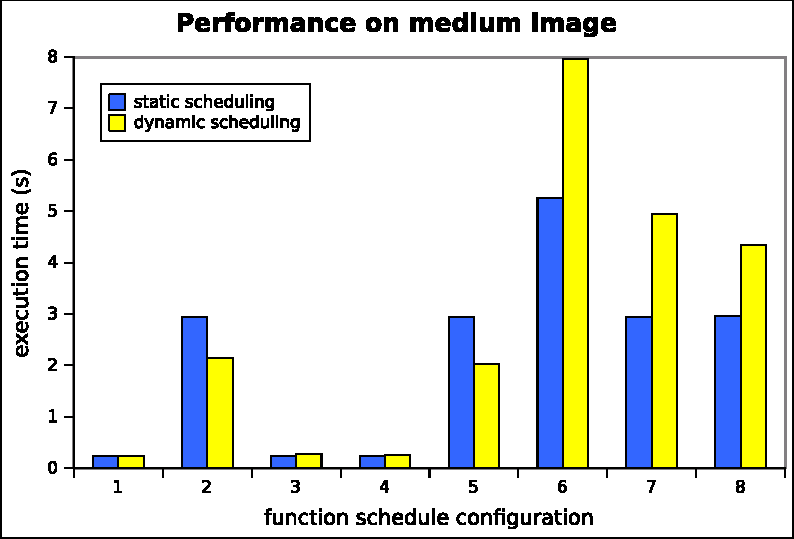
\includegraphics[width=0.7\textwidth]{graphs/medium.pdf}
	\end{center}
\end{frame}

\begin{frame}{Result: Dynamic Scheduling Saves Time (sometimes...)}
	For medium and large images, measured execution time

	\begin{center}
	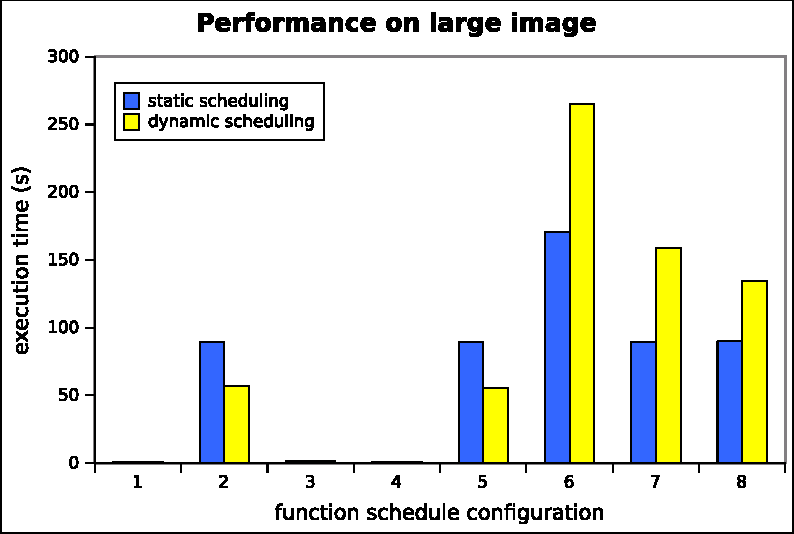
\includegraphics[width=0.7\textwidth]{graphs/large.pdf}
	\end{center}
\end{frame}

\begin{frame}{Which function schedules did I use?}
	\texttt{flipped.tile(x, y, xi, yi, 2, 2);}
	\pause
	\linegap

	\begin{itemize}
		\item \texttt{inverted.store\_at(c)}
		\begin{itemize}
			\item \texttt{.compute\_at(y);} (not included)
			\item \texttt{.compute\_at(x);} (not included)
			\item \texttt{.compute\_at(yi);} (\#1)
			\item \texttt{.compute\_at(xi);} (\#2)
		\end{itemize}
		\item \texttt{inverted.store\_at(y)}
		\begin{itemize}
			\item \texttt{.compute\_at(x);} (\#3)
			\item \texttt{.compute\_at(yi);} (\#4)
			\item \texttt{.compute\_at(xi);} (\#5)
		\end{itemize}
		\item \texttt{inverted.store\_at(x)}
		\begin{itemize}
			\item \texttt{.compute\_at(yi);} (\#6)
			\item \texttt{.compute\_at(xi);} (\#7)
		\end{itemize}
		\item \texttt{inverted.store\_at(yi)}
		\begin{itemize}
			\item \texttt{.compute\_at(xi);} (\#8)
		\end{itemize}
	\end{itemize}
	
\end{frame}

\end{document}

%%%%%%%%%%%%%%%%%%%%%%%%%%%%%%%%%%%%%%%%%%%%%%%%%%%%%%%%%%%%%%%%%%%%%%%%%%%%%%%%
% vim: foldmethod=indent
